\documentclass[10pt,a4paper]{book}
\usepackage[utf8]{inputenc}
\usepackage{amsmath}
\usepackage{amsfonts}
\usepackage{amssymb}
\usepackage{graphicx}
\usepackage[left=3.00cm, right=3.00cm, top=2.00cm, bottom=1.00cm]{geometry}
\usepackage{listings}
\usepackage{xcolor}

\definecolor{codegreen}{rgb}{0,0.6,0}
\definecolor{codegray}{rgb}{0.5,0.5,0.5}
\definecolor{codepurple}{rgb}{0.58,0,0.82}
\definecolor{backcolour}{rgb}{0.95,0.95,0.92}

\lstdefinestyle{mystyle}{
	backgroundcolor=\color{backcolour},   
	commentstyle=\color{codegreen},
	keywordstyle=\color{magenta},
	numberstyle=\tiny\color{codegray},
	stringstyle=\color{codepurple},
	basicstyle=\ttfamily\footnotesize,
	breakatwhitespace=false,         
	breaklines=true,                 
	captionpos=b,                    
	keepspaces=true,                 
	numbers=left,                    
	numbersep=5pt,                  
	showspaces=false,                
	showstringspaces=false,
	showtabs=false,                  
	tabsize=2
}

\lstset{style=mystyle}
\title{Moto dei Razzi}
\date{}
\begin{document}
\noindent{}La generica equazione dei razzi afferma che:
$$
	M\;\frac{d\mathbf v}{dt} = \mathbf{F^{ext}} + \frac{dM}{dt} \mathbf u\;\;\;(1)
$$
Se ci troviamo nella situazione in cui l'interazione gravitazionale tra il razzo e la Terra è non trascurabile, decidiamo di studiare il problema assumendo che:
$$
\mathbf{F^{ext}} = \mathbf{F_p} = - M\;\mathbf g
$$
Supponendo di trovarsi in un sistema di riferimento come quello in figura, allora posso proiettare le grandezze vettoriali lungo la verticale ascendente:
$$
M\;\mathbf g = - M\;g\;\mathbf j
$$
$$
\mathbf v = v\;\mathbf j
$$
$$
\mathbf u = u\;\mathbf j
$$
A questo punto è possibile riscrivere la $(1)$ come segue:
$$
	M\;\frac{dv}{dt} = M\;g + \frac{dM}{dt} u\;\;\;(2)
$$
\begin{figure}[h]
	\centering
	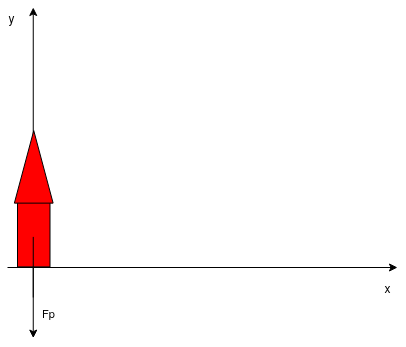
\includegraphics[width=0.7\linewidth]{rocket.png}
	\label{fig:rocket}
\end{figure}\\*
La soluzione nota della $(2)$:
$$
v_f = v_i - g(t_f-t_0) + u\;\log\left(\frac{m_i}{m_f}\right)
$$
È valida sotto l'assunzione che la forza peso $F_p$ del razzo all'istante $t$ sia sempre pari alla sua massa all'istante $t$ moltiplicata per $-g$:
$$
F_p = -M(t)\;g\;\;\;\;g \approx 9.81 \frac{m}{s^2}
$$
Ovvero consideriamo costante l'accelerazione di gravità.\newpage\noindent{}Quello che mi domandavo io, è che noi conosciamo un modello abbastanza semplice che ci permette di determinare la reciproca forza attrattiva tra due punti nello spazio, cioè la legge di gravitazione universale. In particolare, se $M$ è la massa del razzo a un certo istante $t$, $M_t$ è la massa della Terra, e $d$ la distanza tra i centri di massa  della Terra e del razzo:
$$
\mathbf{F_{Terra\rightarrow razzo}} = -G \frac{MM_t}{d^2}\;\mathbf j\;\;\;(3)
$$
Supponendo che all'istante $t=0$ valga $y(0)=R_t$, con $R_t$ raggio della Terra, potrei riscrivere la $(3)$ in funzione della coordinata $y$:
$$
\mathbf{F_{Terra\rightarrow razzo}} = -G \frac{MM_t}{y^2}\;\mathbf j
$$
Andando a sostituire nella $(1)$ proiettata sull'asse $y$, ottengo:
$$
	M\;\frac{dv}{dt} = -G \frac{MM_t}{y^2}- \frac{dM}{dt} u\;\;\;(4)
$$
Considerando che:
$$
\frac{dv}{dt} = a = \ddot{y}
$$
$$
\frac{dM}{dt} = \dot{M}
$$
Potrei nuovamente riscrivere la $(4)$:
$$
M \ddot{y} = -G \frac{MM_t}{y^2} - \dot{M} u
$$
$$
\ddot{y} = -G \frac{M_t}{y^2} - \frac{\dot{M}}{M} u
$$
$$
\ddot{y} = (-G\;M_t) \frac{1}{y^2} - \frac{\dot{M}}{M} u
$$
Ponendo $\alpha = -G\;M_t$:
$$
\ddot{y} = \alpha \frac{1}{y^2} - \frac{\dot{M}}{M} u\;\;\;(5)
$$
Quello che ho pensato è che $dM = -dm$ è la quantità di gas espulso cambiata di segno, è costante e dipende esclusivamente dalla chimica del processo di combustione, e non dalla coordinata $y$. In generale per la massa $M$ del razzo vale:
$$
M(t) = m_{mec}(t) + m_{carb}(t)
$$
$$
M(t+dt) = m_{mec}(t+dt) + m_{carb}(t + dt)
$$
La $m_{mec}$ del razzo rimane sempre costante (a meno di considerare eventuali stadi), mentre ciò che varia è $m_{carb}$. Quindi posso scrivere:
$$
M(t+dt) = m_{mec}(t) + m_{carb}(t + dt)
$$
$$
M(t+dt) = m_{mec}(t) + m_{carb}(t) - dm
$$
Di conseguenza:
$$
\dot M = \frac{dM}{dt} = \frac{M(t + dt) - M(t)}{dt} = \frac{m_{mec}(t) + m_{carb}(t) - dm - m_{mec}(t) - m_{carb}(t) }{dt}
= -\frac{dm}{dt}$$ 
La quantità $\frac{dm}{dt}$ è il rate di espulsione del gas, che sappiamo essere costante a parità di processo chimico:
$$
\frac{dm}{dt} = k > 0
$$
Quindi:
$$
\frac{dM}{dt} = -\frac{dm}{dt} \Rightarrow \frac{dM}{dt} = -k\;\;\;(6)
$$
\newpage\noindent{}
La $(6)$ è una equazione differenziale lineare del primo ordine a coefficienti costanti, la cui soluzione vale:
$$
M(t) = c - kt
$$
Per trovare $c$ posso risolvere il problema ai valori iniziali:
$$
M(0) = m_{mec} + m_{0_{carb}} 
$$
Dove $m_{mec}$ è la massa delle parti meccaniche del razzo, mentre $m_{0_{carb}}$ è la massa iniziale di carburante:
$$
c - 0k = m_{mec} + m_{0_{carb}} \Rightarrow c = m_{mec} + m_{0_{carb}}
$$
Quindi:
$$
\frac{\dot M}{M} = -\frac{k}{c + kt}
$$
La $(5)$ diventa:
$$
\ddot{y} = \alpha \frac{1}{y^2} + \frac{k}{c + kt} u
$$
Ossia una equazione differenziale non lineare del secondo ordine, la cui soluzione esplicita non penso di saper calcolare; ma che posso comunque approssimare numericamente.
\begin{lstlisting}[language=MATLAB]
function dydt = rocket(t,y,a,c,k)
	dydt = zeros(2,1);
	dydt(1) = y(2);
	dydt(2) = (k/(c+k*t.))*a*1/y(1)^2;

G = 6.67*1e-11;
Mt = 6e24;
a = (-G*Mt);
c = 7000; #7000kg di carburante
k = 100; #100kg al secondo
tspan = [0 5];
y0 = [0 0.01];
[t,y] = ode45(@(t,y) rocket(t,y,a,c,k), tspan, y0);
plot(t,y(:,1),'-o',t,y(:,2),'-.');
\end{lstlisting}
\newpage
\begin{tabular}{|l|l|l|}
	\hline 
	\textbf{Distanza centro Terra (m)}&\textbf{Distanza superficie terrestre (m)}&\textbf{Stima di g (m/$\mathbf{s^2}$)} \\ 
	\hline 
$6.371000\;10^6$ & $0.000000\;10^0$ & $-10.0211$ \\
\hline
$6.376448\;10^6$ & $5.447722\;10^3$ & $-10.0211$ \\
\hline
$6.392830\;10^6$ & $2.183007\;10^4$ & $-9.9869$ \\
\hline
$6.420206\;10^6$ & $4.920630\;10^4$ & $-9.9188$ \\
\hline
$6.458636\;10^6$ & $8.763636\;10^4$ & $-9.8177$ \\
\hline
$6.508181\;10^6$ & $1.371809\;10^5$ & $-9.685$ \\
\hline
$6.568901\;10^6$ & $1.979012\;10^5$ & $-9.5224$ \\
\hline
$6.640859\;10^6$ & $2.698594\;10^5$ & $-9.3322$ \\
\hline
$6.724118\;10^6$ & $3.531181\;10^5$ & $-9.1167$ \\
\hline
$6.818741\;10^6$ & $4.477409\;10^5$ & $-8.8789$ \\
\hline
$6.924792\;10^6$ & $5.537920\;10^5$ & $-8.6216$ \\
\hline
$7.042336\;10^6$ & $6.713362\;10^5$ & $-8.3478$ \\
\hline
$7.171439\;10^6$ & $8.004394\;10^5$ & $-8.0606$ \\
\hline
$7.312168\;10^6$ & $9.411680\;10^5$ & $-7.7631$ \\
\hline
$7.464589\;10^6$ & $1.093589\;10^6$ & $-7.4583$ \\
\hline
$7.628771\;10^6$ & $1.257771\;10^6$ & $-7.1488$ \\
\hline
$7.804782\;10^6$ & $1.433782\;10^6$ & $-6.8371$ \\
\hline
$7.992692\;10^6$ & $1.621692\;10^6$ & $-6.5257$ \\
\hline
$8.192572\;10^6$ & $1.821572\;10^6$ & $-6.2168$ \\
\hline
$8.404492\;10^6$ & $2.033492\;10^6$ & $-5.9121$ \\
\hline
$8.628525\;10^6$ & $2.257525\;10^6$ & $-5.6136$ \\
\hline
$8.864744\;10^6$ & $2.493744\;10^6$ & $-5.3221$ \\
\hline
$9.113223\;10^6$ & $2.742223\;10^6$ & $-5.0389$ \\
\hline
$9.374035\;10^6$ & $3.003035\;10^6$ & $-4.765$ \\
\hline
$9.647257\;10^6$ & $3.276257\;10^6$ & $-4.5013$ \\
\hline
$9.932966\;10^6$ & $3.561966\;10^6$ & $-4.248$ \\
\hline
$1.023124\;10^7$ & $3.860238\;10^6$ & $-4.0056$ \\
\hline
$1.054215\;10^7$ & $4.171153\;10^6$ & $-3.7741$ \\
\hline
$1.086579\;10^7$ & $4.494789\;10^6$ & $-3.5536$ \\
\hline
$1.120223\;10^7$ & $4.831227\;10^6$ & $-3.3442$ \\
\hline
$1.155155\;10^7$ & $5.180548\;10^6$ & $-3.1457$ \\
\hline
$1.191383\;10^7$ & $5.542834\;10^6$ & $-2.9578$ \\
\hline
$1.228917\;10^7$ & $5.918170\;10^6$ & $-2.7802$ \\
\hline
$1.267764\;10^7$ & $6.306639\;10^6$ & $-2.6127$ \\
\hline
$1.307933\;10^7$ & $6.708326\;10^6$ & $-2.4549$ \\
\hline
$1.349432\;10^7$ & $7.123320\;10^6$ & $-2.3063$ \\
\hline
$1.392271\;10^7$ & $7.551707\;10^6$ & $-2.1666$ \\
\hline
$1.436458\;10^7$ & $7.993576\;10^6$ & $-2.0353$ \\
\hline
$1.482002\;10^7$ & $8.449017\;10^6$ & $-1.9121$ \\
\hline
$1.528912\;10^7$ & $8.918123\;10^6$ & $-1.7964$ \\
\hline
$1.577198\;10^7$ & $9.400985\;10^6$ & $-1.688$ \\
\hline
$1.626870\;10^7$ & $9.897697\;10^6$ & $-1.5864$ \\
\hline
$1.677935\;10^7$ & $1.040835\;10^7$ & $-1.4911$ \\
\hline
$1.730405\;10^7$ & $1.093305\;10^7$ & $-1.4019$ \\
\hline
$1.784289\;10^7$ & $1.147189\;10^7$ & $-1.3183$ \\
\hline
$1.839597\;10^7$ & $1.202497\;10^7$ & $-1.2401$ \\
\hline
$1.896338\;10^7$ & $1.259238\;10^7$ & $-1.1668$ \\
\hline
$1.954524\;10^7$ & $1.317424\;10^7$ & $-1.0982$ \\
\hline
$2.014164\;10^7$ & $1.377064\;10^7$ & $-1.0339$ \\
\hline
$2.075269\;10^7$ & $1.438169\;10^7$ & $-0.97378$ \\
\hline
$2.137850\;10^7$ & $1.500750\;10^7$ & $-0.91743$ \\
\hline
$2.201917\;10^7$ & $1.564817\;10^7$ & $-0.86466$ \\
\hline
$2.267481\;10^7$ & $1.630381\;10^7$ & $-0.81523$ \\
\hline
$2.334553\;10^7$ & $1.697453\;10^7$ & $-0.76892$ \\
\hline
$2.403145\;10^7$ & $1.766045\;10^7$ & $-0.72551$ \\
\hline
$2.473269\;10^7$ & $1.836169\;10^7$ & $-0.68481$ \\
\hline
$2.544935\;10^7$ & $1.907835\;10^7$ & $-0.64665$ \\
\hline
$2.618155\;10^7$ & $1.981055\;10^7$ & $-0.61086$ \\
\hline
$2.692942\;10^7$ & $2.055842\;10^7$ & $-0.5773$ \\
\hline
$2.769308\;10^7$ & $2.132208\;10^7$ & $-0.54578$ \\
\hline

\end{tabular} 
\end{document}
